Nesta seção, são apresentados os materiais e métodos utilizados no desenvolvimento do sistema. Isso inclui as ferramentas e tecnologias empregadas, a arquitetura do sistema e as integrações realizadas.

\section{Descrição da área de estudo}
O sistema em questão foi implementado no Instituto Federal de Minas Gerais (IFMG), \textit{Campus} Bambuí, especificamente no Laboratório de Sistemas Embarcados. Esse local foi escolhido por possuir uma infraestrutura adequada para o teste de sensores e equipamentos necessários para a captura e transmissão de dados. A escolha do laboratório também se deve à disponibilidade de supervisão técnica e apoio logístico para a instalação e validação dos equipamentos.

\section{Classificação da pesquisa}

A pesquisa realizada no desenvolvimento do sistema de monitoramento meteorológico pode ser classificada segundo os seguintes critérios: quanto aos objetivos, à natureza, aos procedimentos técnicos e à abordagem do problema.

\subsection{Quanto aos objetivos}

De acordo com os objetivos, esta pesquisa é classificada como descritiva e exploratória. 

A pesquisa é descritiva porque visa descrever as características dos fenômenos meteorológicos monitorados pelos sensores, bem como o comportamento do sistema de monitoramento implementado. O foco foi detalhar como as variáveis meteorológicas, como temperatura, umidade, pressão, velocidade do vento e luminosidade, são capturadas e processadas pelo sistema, além de documentar o desempenho dos componentes de \textit{hardware} e \textit{software} utilizados.

A pesquisa também é exploratória porque busca investigar a aplicabilidade e eficiência de diferentes tecnologias e métodos no monitoramento meteorológico. Isso inclui a experimentação com diversos sensores e técnicas de integração de dados em um contexto específico. O caráter exploratório é acentuado pela busca de soluções tecnológicas que possam ser escaláveis e aplicáveis a diferentes contextos de monitoramento ambiental.

\subsection{Quanto à natureza}

Quanto à natureza, a pesquisa é aplicada. O objetivo principal foi o desenvolvimento de uma solução prática para um problema real, neste caso, a necessidade de monitoramento meteorológico em tempo real. O conhecimento gerado é voltado para a aplicação direta no sistema desenvolvido, com o propósito de melhorar a coleta, processamento e análise de dados meteorológicos. A pesquisa aplicada busca, portanto, transformar o conhecimento teórico em soluções práticas e funcionais.

\subsection{Quanto aos procedimentos técnicos}

Em relação aos procedimentos técnicos, a pesquisa é classificada como experimental. Durante o desenvolvimento do sistema, foram realizados testes e experimentos com diferentes componentes \textit{hardware} e \textit{software}, a fim de avaliar seu desempenho e adequação ao monitoramento meteorológico. Esses testes incluíram a validação dos sensores, a integração com o microcontrolador ESP32 e a transmissão de dados através do protocolo MQTT. A pesquisa experimental permitiu ajustes e refinamentos no sistema até alcançar um protótipo funcional e validado.

\subsection{Quanto à abordagem do problema}

Quanto à abordagem do problema, esta pesquisa é qualitativa. O sistema desenvolvido coleta, processa e fornece dados meteorológicos numéricos que são quantificados e apresentados em \textit{cards} interativos. Isso é feito por meio de uma interface de visualização com os dados capturados pelos sensores. Assim, foi possível a observação de variáveis como temperatura, umidade, pressão e velocidade do vento, além de possibilitar o cálculo de índices climáticos, como a evapotranspiração. A abordagem qualitativa foi escolhida como forma de interpretar os dados meteorológicos de maneira específica para cada área de coleta, permitindo uma análise detalhada das variáveis ambientais em seus contextos locais. Essa especificidade garante que os dados reflitam as condições e particularidades de cada região, favorecendo uma compreensão fundamentada dos fenômenos climáticos estudados.

\section{Componentes do Sistema de Monitoramento Meteorológico}

O sistema desenvolvido utiliza uma série de sensores para monitorar em tempo real diferentes parâmetros meteorológicos. Nesta seção, são apresentados os sensores e módulos utilizados no sistema, suas funcionalidades, características principais e como foram integrados ao microcontrolador ESP32 para a coleta e transmissão de dados meteorológicos.

\subsection{Sensor de Temperatura e Umidade DHT22}

O sensor DHT22 (Figura \ref{figura:dht22}) mede a temperatura e a umidade do ar, com precisão dentro do intervalo de operação \parencite{DHT22}. O pino de saída do sensor foi conectado ao pino GPIO 4 do ESP32, configurado no código como \texttt{DHTPIN}. Para alimentação, o sensor foi conectado ao pino 3V3 e ao GND do ESP32. Na Tabela \ref{tab:dht22}, são apresentadas as especificações técnicas do sensor.

O uso do sensor DHT22 no sistema justifica-se pela sua precisão dentro da faixa de operação desejada, característica necessária para o monitoramento climático \parencite{DHT22}. A medição precisa de temperatura e umidade relativa do ar é indispensável em aplicações meteorológicas, pois esses parâmetros influenciam diretamente fenômenos atmosféricos e condições ambientais. Além disso, a facilidade de integração ao ESP32 por meio de um único pino digital reduz a complexidade do circuito, otimizando a implementação do sistema. A escolha do DHT22, em detrimento de outros sensores, também considera o seu equilíbrio entre custo-benefício e desempenho, sendo utilizado em projetos de monitoramento ambiental \parencite{ferrandez2018precision,Francisco_precision2024}.

\begin{figure}[!htb] \centering
  \caption{Sensor de temperatura e umidade DHT22} \label{figura:dht22}
  \begin{varwidth}{\linewidth}
    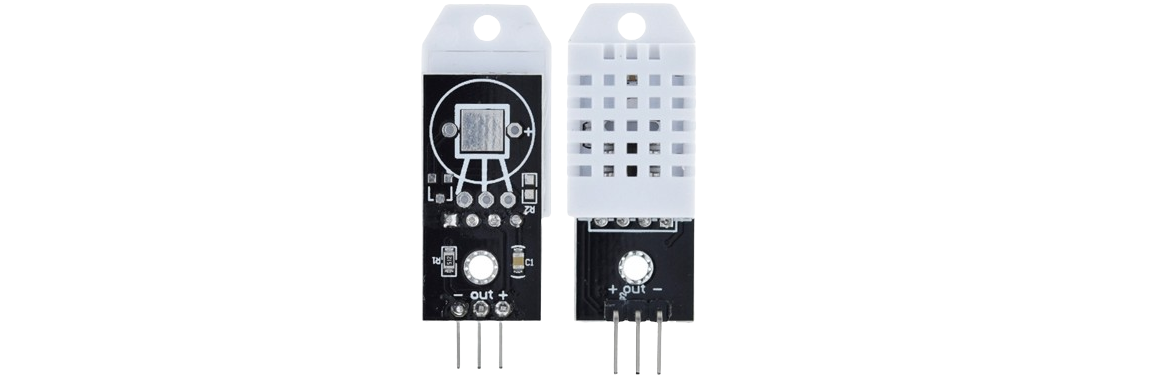
\includegraphics[width=16cm]{figuras/DHT22.png}
    \fonte{Retirado de \textcite{DHT22}.}
  \end{varwidth}
\end{figure}

\begin{table}[!htb]
    \caption{Especificações técnicas do sensor DHT22}
    \begin{tabularx}{\textwidth}{|X|X|} \hline
        \textbf{Parâmetro} & \textbf{Detalhes} \\ \hline
        Faixa de operação & Umidade: 0-100\% RH; Temperatura: -40\textdegree C a 80\textdegree C \\ \hline
        Precisão & Umidade: $\pm$2\% RH (Máx $\pm$5\%RH); Temperatura: $<$ $\pm$0.5\textdegree C \\ \hline
        Resolução/Sensibilidade & Umidade: 0.1\% RH; Temperatura: 0.1\textdegree C \\ \hline
        Período de amostragem & Média: 2 s \\ \hline
        Dimensões & 22x28x5 mm \\ \hline
    \end{tabularx}
    \label{tab:dht22}
    \fonte{Retirado de \textcite{DHT22}.}
\end{table}

\subsection{Sensor de Pressão BMP280}

O sensor BMP280 (Figura \ref{figura:bmp280}) mede a pressão atmosférica com precisão, além de oferecer medições de temperatura \parencite{BMP280}. Ele utiliza o barramento I2C, sendo conectado aos pinos padrão do ESP32 para \texttt{SDA} e \texttt{SCL}. Para alimentação, o sensor também foi conectado ao pino 3V3 e ao GND do ESP32. Na Tabela \ref{tab:bmp280}, são apresentadas as especificações técnicas do sensor.

A inclusão do sensor BMP280 no sistema deve-se à sua capacidade de medir pressão atmosférica com precisão, o que é necessário para a análise de condições meteorológicas e a previsão de mudanças climáticas \parencite{BMP280}. A pressão atmosférica é um parâmetro utilizado na modelagem de padrões climáticos, e o BMP280 oferece dados confiáveis dentro de uma faixa de operação desejada, adequado tanto para altitudes elevadas quanto para ambientes ao nível do mar. Além disso, a integração por barramento I2C simplifica a comunicação com o microcontrolador ESP32, permitindo o compartilhamento de pinos com outros dispositivos. A resolução do sensor possibilita a detecção de variações sutis na pressão, úteis para aplicações detalhadas, como estudos de microclimas \parencite{Prathibha_system2017, Lamine_precision2024}.

\begin{figure}[!htb] \centering
  \caption{Sensor de pressão barométrica BMP280} \label{figura:bmp280}
  \begin{varwidth}{\linewidth}
    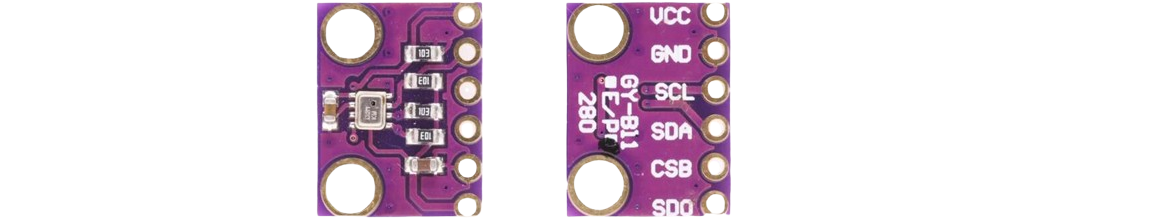
\includegraphics[width=16cm]{figuras/BMP280.png}
    \fonte{Retirado de \textcite{BMP280}.}
  \end{varwidth}
\end{figure}

\begin{table}[!htb]
  \caption{Especificações técnicas do sensor BMP280}
  \begin{tabularx}{\textwidth}{|X|X|} \hline
      \textbf{Parâmetro} & \textbf{Detalhes} \\ \hline
      Faixa de operação & 300-1100 hPa \\ \hline
      Precisão absoluta & $\sim$ $\pm$1 hPa (950-1050 hPa) \\ \hline
      Precisão relativa & $\pm$0.12 hPa (700-900 hPa) \\ \hline
      Resolução/Sensibilidade & 0.01 hPa (< 10 cm) \\ \hline
      Período de amostragem & Média: 5.5 ms \\ \hline
      Dimensões & 8x15.62x0.85 mm \\ \hline
  \end{tabularx}
  \label{tab:bmp280}
  \fonte{Retirado de \textcite{BMP280}.}
\end{table}

\subsection{Sensor de Luminosidade BH1750}

O BH1750 (Figura \ref{figura:bh1750}) é um sensor digital de luminosidade que mede a intensidade luminosa em lux. Ele também utiliza o barramento I2C, compartilhando os mesmos pinos do BMP280. Para alimentação, o sensor também foi conectado ao pino 3V3 e ao GND do ESP32. Na Tabela \ref{tab:bh1750}, são apresentadas as especificações técnicas do sensor.

A escolha do sensor BH1750 é justificada por sua capacidade de medir a intensidade luminosa em lux, unidade aceita no estudo da iluminação ambiental e solar \parencite{Prathibha_system2017,Vijh_system2024, Amine_system2024}. A intensidade luminosa afeta diversos processos meteorológicos e biológicos, como evaporação e fotossíntese, tornando sua medição uma parte integrante do monitoramento climático \parencite{Yang_evapotranspiration_med2022}. O BH1750 destaca-se por sua sensibilidade, faixa de operação e comunicação digital por I2C, que asseguram medições rápidas e precisas \parencite{BH1750}. Além disso, a possibilidade de alternar entre modos de alta e baixa resolução adapta-se às necessidades específicas do sistema, proporcionando flexibilidade na coleta de dados.

\begin{figure}[!htb] \centering
  \caption{Sensor de luminosidade BH1750} \label{figura:bh1750}
  \begin{varwidth}{\linewidth}
    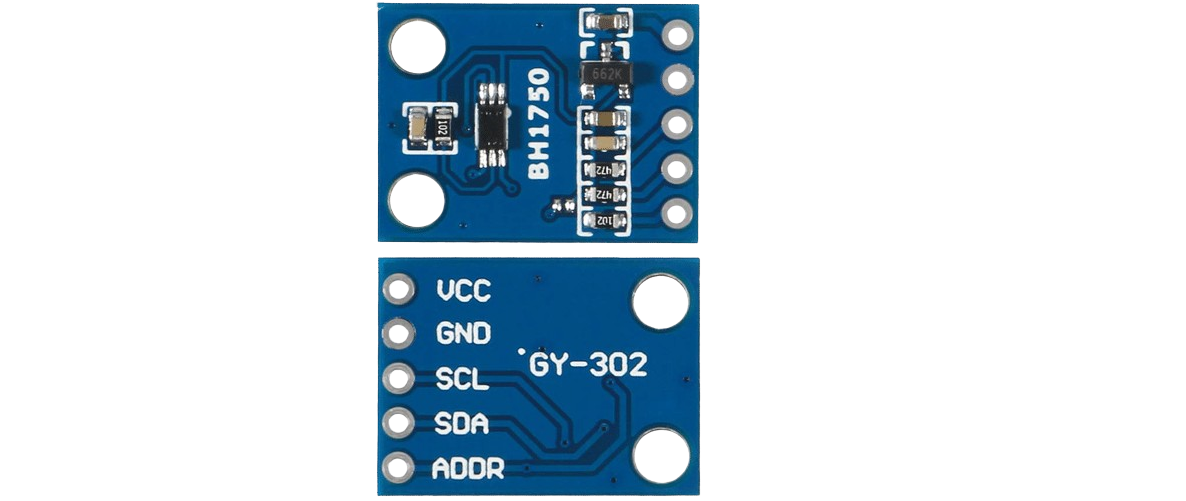
\includegraphics[width=16cm]{figuras/BH1750.png}
    \fonte{Retirado de \textcite{BH1750}.}
  \end{varwidth}
\end{figure}

\begin{table}[!htb]
    \caption{Especificações técnicas do sensor BH1750}
    \begin{tabularx}{\textwidth}{|X|X|} \hline
        \textbf{Parâmetro} & \textbf{Detalhes} \\ \hline
        Faixa de operação & 0-65535 lx \\ \hline
        Precisão & $\pm$0.24 lx  \\ \hline
        Resolução/Sensibilidade & Alta Resolução: 1 lx; Baixa Resolução: 4 lx \\ \hline
        Período de amostragem & Alta Resolução: 120-180 ms; Baixa Resolução: 16-24 ms \\ \hline
        Dimensões & 13.9x18.5 mm \\ \hline
    \end{tabularx}
    \label{tab:bh1750}
    \fonte{Retirado de \textcite{BH1750}.}
\end{table}

\subsection{Anemômetro RS-FSJT-N01}

O anemômetro RS-FSJT-N01 (Figura \ref{figura:anemometro}) é utilizado para medir a velocidade do vento. Ele opera por meio do protocolo Modbus RTU sobre RS485, enviando os dados de velocidade em m/s. Para a integração ao ESP32, foi necessário o uso do módulo conversor RS485 para TTL, que possibilita a comunicação compatível com os níveis lógicos do microcontrolador. Na Tabela \ref{tab:anemometro}, são apresentadas as especificações técnicas do anemômetro.

O anemômetro RS-FSJT-N01 foi selecionado devido à sua precisão na medição da velocidade do vento, um dos parâmetros utilizados em estudos meteorológicos e ambientais \parencite{Prathibha_system2017,Amine_system2024}. A velocidade do vento influencia diretamente fenômenos como a dispersão de poluentes, a sensação térmica e o transporte de umidade na atmosfera \parencite{Zhang_evapotranspiration_med2016}. Este modelo específico utiliza o protocolo Modbus RTU sobre RS485, uma tecnologia que garante comunicação confiável em ambientes sujeitos a ruído eletromagnético \parencite{ANEMOMETER}.

\begin{figure}[!htb] \centering
  \caption{Anemômetro RS-FSJT-N01} \label{figura:anemometro}
  \begin{varwidth}{\linewidth}
    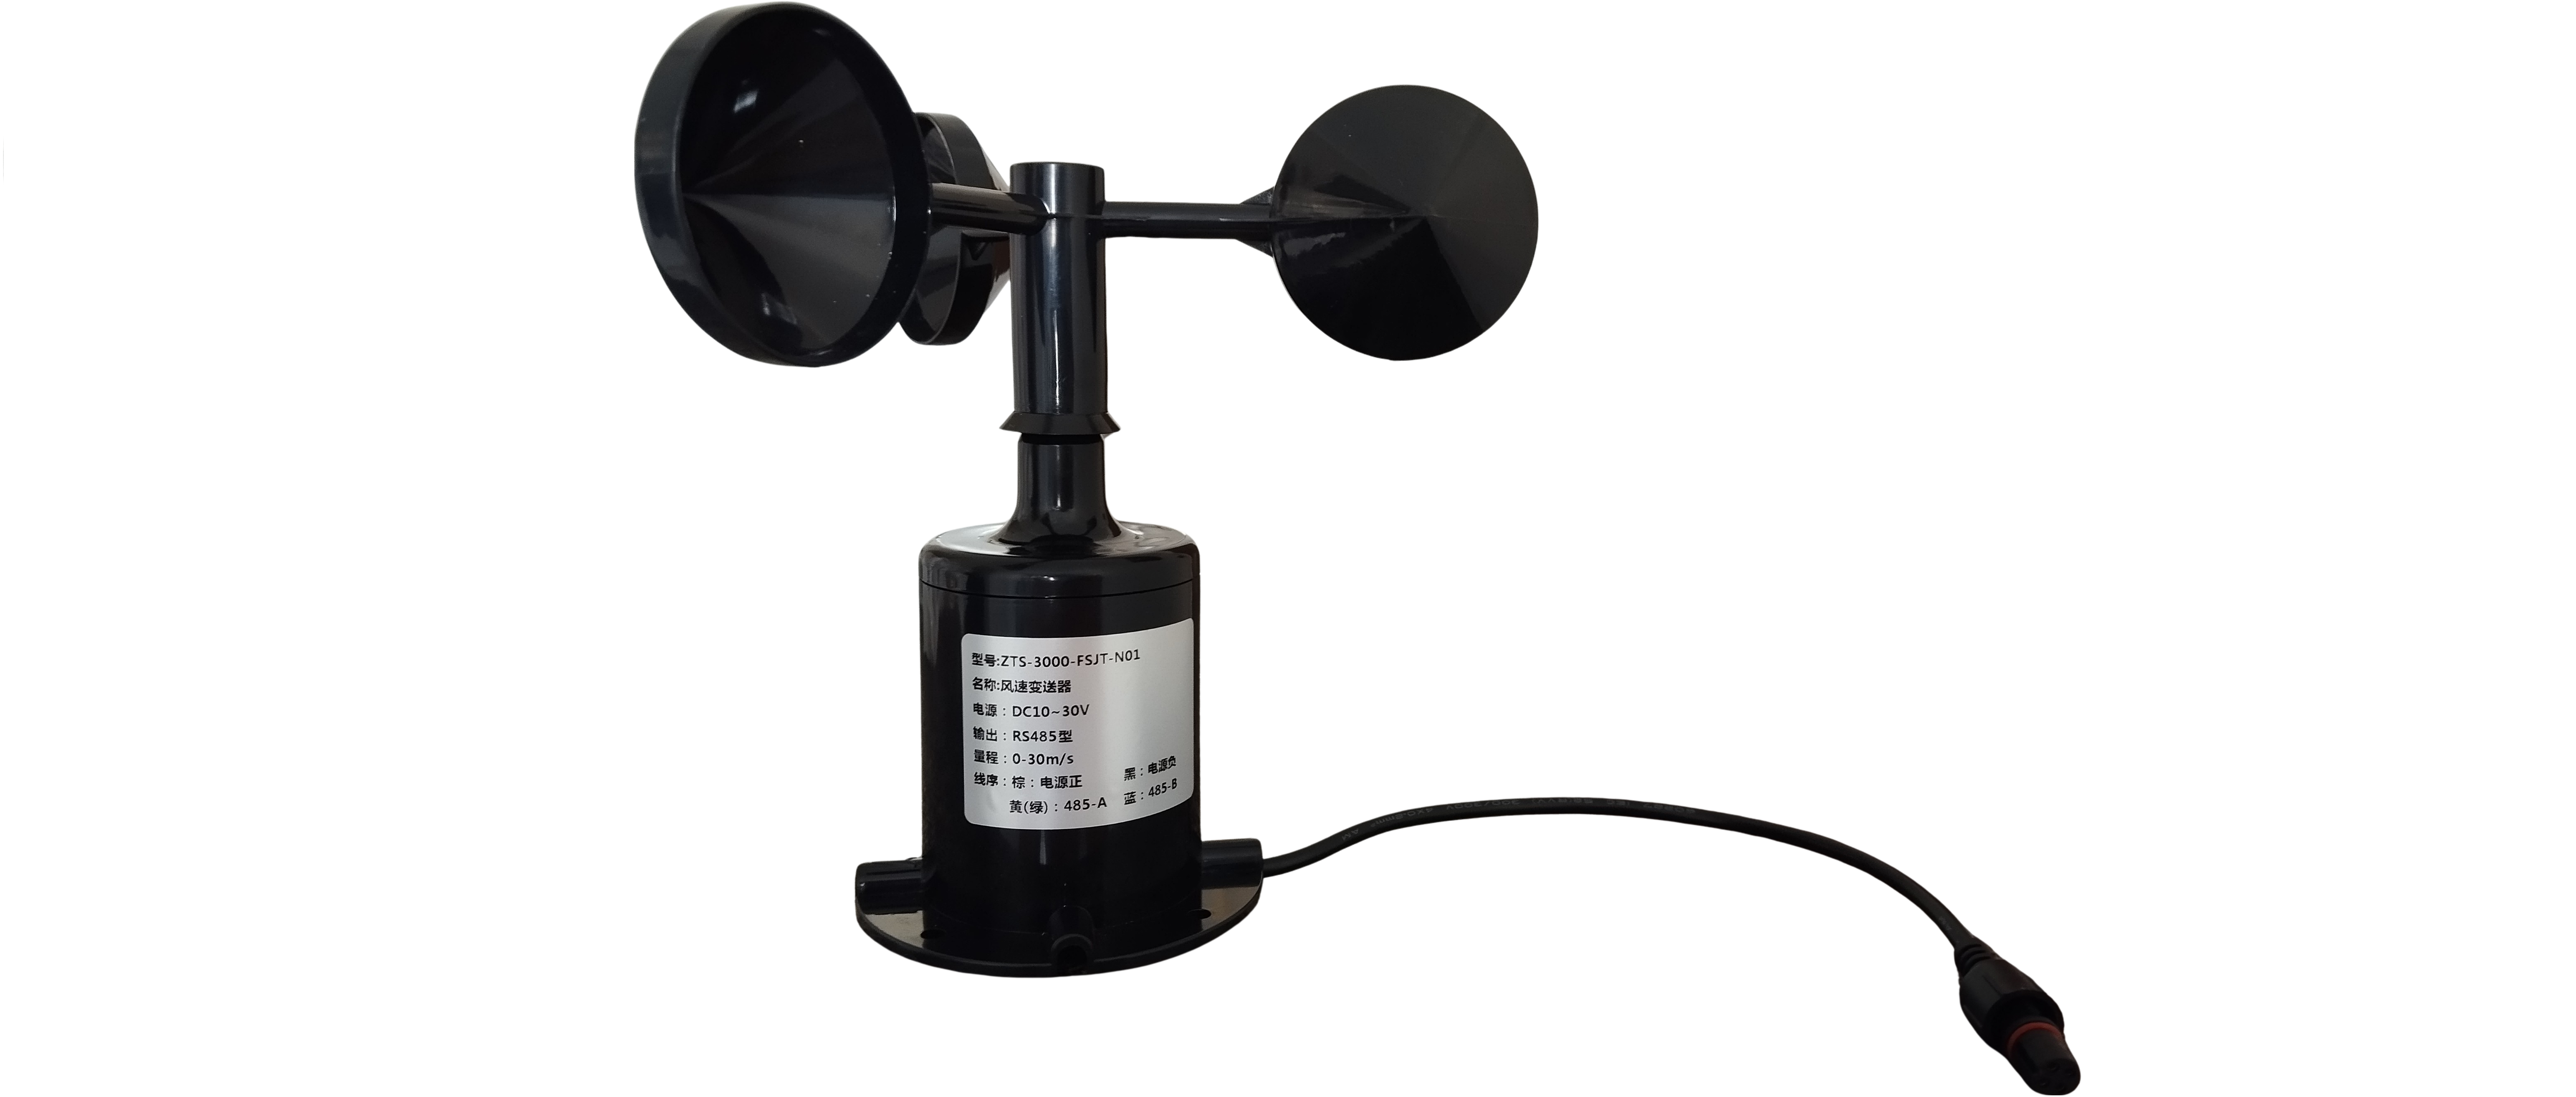
\includegraphics[width=16cm]{figuras/Anemometer.png}
    \fonte{Retirado de \textcite{ANEMOMETER}.}
  \end{varwidth}
\end{figure}

\begin{table}[!htb]
    \caption{Especificações técnicas do Anemômetro RS-FSJT-N01}
    \begin{tabularx}{\textwidth}{|X|X|} \hline
        \textbf{Parâmetro} & \textbf{Detalhes} \\ \hline
        Faixa de operação & 0-30 m/s \\ \hline
        Precisão & $\pm$0.3 m/s  \\ \hline
        Resolução/Sensibilidade & 0.1 m/s \\ \hline
        Período de amostragem & $\leq$ 1 s \\ \hline
        Dimensões & 182x80x160 mm \\ \hline
    \end{tabularx}
    \label{tab:anemometro}
    \fonte{Retirado de \textcite{ANEMOMETER}.}
\end{table}

\subsection{Comparador de Umidade do Solo LM393}

O módulo LM393 (Figura \ref{figura:lm393}) detecta a presença de umidade no solo com base na variação de condutividade elétrica. Ele foi conectado ao pino GPIO 13 do ESP32, configurado como entrada digital. Para alimentação, o módulo foi conectado ao pino 3V3 e ao GND do ESP32.

Para solos úmidos (acima de 50\% de umidade), o módulo fornece um sinal digital baixo (0), enquanto, para solos secos (abaixo de 50\% de umidade), o sinal é alto (1). O limiar de umidade pode ser ajustado através do potenciômetro presente no módulo usando-se uma chave \textit{philips}.

O comparador LM393 foi escolhido por ser ajustável e sensível a variações de umidade no solo \parencite{LM393}. A umidade do solo é um fator importante no contexto da irrigação, influenciando diretamente a absorção de nutrientes pelas plantas \parencite{Zhang_evapotranspiration_med2016}. O LM393 permite a detecção rápida e precisa de mudanças na umidade do solo, tornando a coleta em tempo real mais eficiente. Na Tabela \ref{tab:lm393}, são apresentadas as especificações técnicas do comparador.

\begin{figure}[!htb] \centering
  \caption{Comparador de umidade do solo LM393} \label{figura:lm393}
  \begin{varwidth}{\linewidth}
    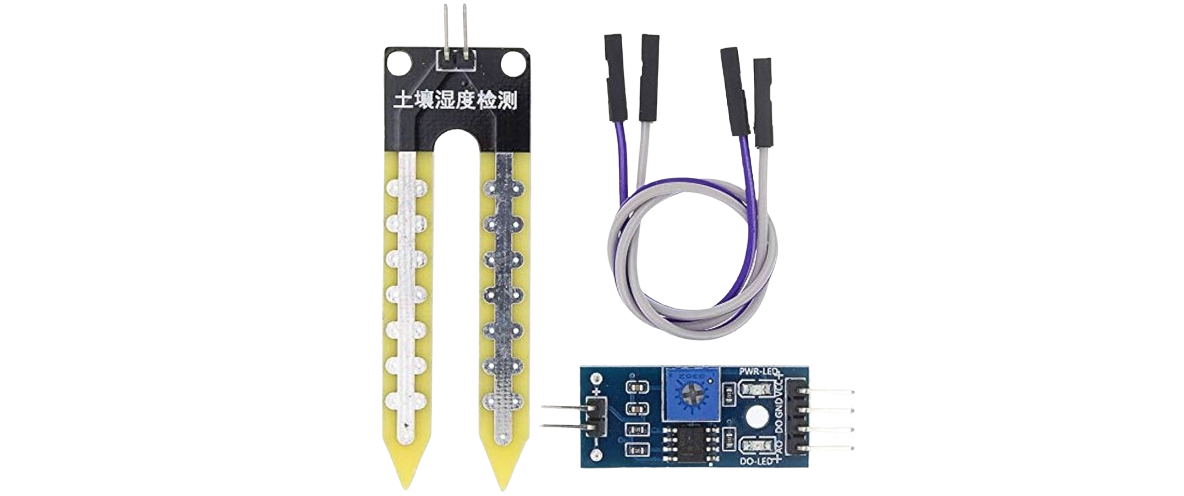
\includegraphics[width=16cm]{figuras/LM393.png}
    \fonte{Retirado de \textcite{LM393}.}
  \end{varwidth}
\end{figure}

\begin{table}[!htb]
  \caption{Especificações técnicas do Comparador LM393}
  \begin{tabularx}{\textwidth}{|X|X|} \hline
      \textbf{Parâmetro} & \textbf{Detalhes} \\ \hline
      Faixa de operação & 2.0 V a 36 V \\ \hline
      Precisão & $\pm$5.0 mV \\ \hline
      Resolução/Sensibilidade & 5 nA (corrente de offset) \\ \hline
      Período de amostragem & $\leq$ 1.3 $\mu$s \\ \hline
      Dimensões & 99x16 mm \\ \hline
  \end{tabularx}
  \label{tab:lm393}
  \fonte{Retirado de \textcite{LM393}.}
\end{table}

\subsection{Módulo GPS NEO-6M V2}

O módulo GPS NEO-6M (Figura \ref{figura:neo6m}) fornece informações de localização (latitude, longitude e altitude). Ele foi conectado ao ESP32 utilizando-se os pinos GPIO 18 e 19 para TX e RX, respectivamente. No código, os pinos foram configurados como \texttt{RX0} e \texttt{TX0}, empregando-se o protocolo UART para comunicação serial. Para alimentação, o módulo também foi conectado ao pino 3V3 e ao GND do ESP32.

O módulo GPS NEO-6M foi escolhido por sua capacidade de obtenção de coordenadas geográficas \parencite{NEO6M}. Essa funcionalidade permite a correlação de dados meteorológicos com a posição geográfica, facilitando a análise de padrões climáticos \parencite{Zhang_evapotranspiration_med2016}. O NEO-6M oferece uma precisão de até 2.5 metros, adequada para aplicações que requerem um rastreio preciso da localização \parencite{NEO6M}. Na Tabela \ref{tab:neo6}, são apresentadas as especificações técnicas do módulo.

\begin{figure}[!htb] \centering
  \caption{Módulo GPS NEO-6M V2} \label{figura:neo6m}
  \begin{varwidth}{\linewidth}
    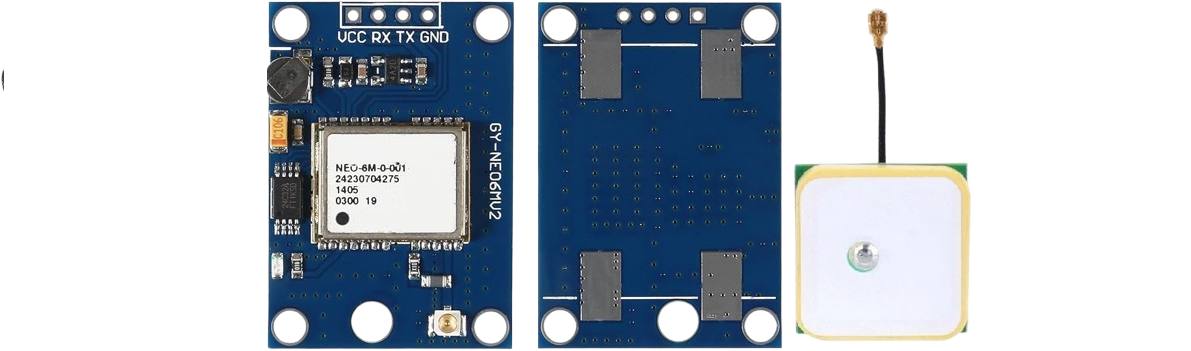
\includegraphics[width=16cm]{figuras/NEO6MV2.png}
    \fonte{Retirado de \textcite{NEO6M}.}
  \end{varwidth}
\end{figure}

\begin{table}[!htb]
  \caption{Especificações técnicas do Módulo GPS NEO-6M V2}
  \begin{tabularx}{\textwidth}{|X|X|} \hline
      \textbf{Parâmetro} & \textbf{Detalhes} \\ \hline
      Faixa de operação & 2.7 V a 3.6 V \\ \hline
      Precisão & 2.5 m (GPS), 2.0 m (SBAS) \\ \hline
      Resolução/Sensibilidade & -161 dBm \\ \hline
      Período de amostragem & Até 5 Hz \\ \hline
      Dimensões & 16x12.2x2.4 mm \\ \hline
  \end{tabularx}
  \label{tab:neo6}
  \fonte{Retirado de \textcite{NEO6M}.}
\end{table}

\subsection{Módulo Conversor RS485 para TTL}

O módulo conversor RS485 para TTL (Figura \ref{figura:ttl_rs485}) é utilizado para conectar o ESP32 ao anemômetro RS-FSJT-N01, convertendo os sinais TTL para níveis compatíveis com RS485 \parencite{RS485TTL}. Ele foi conectado ao ESP32 usando-se os pinos GPIO 16 e 17 (TX e RX), que eram ligados aos pinos RXD e TXD do módulo, respectivamente. Já o barramento RS485 do anemômetro conectado aos terminais A e B do módulo e a alimentação deste foram feitos por uma fonte de 12V genérica. No código, os pinos foram configurados como \texttt{MAX485\_RX} e \texttt{MAX485\_TX}, para a comunicação serial. Na Tabela \ref{tab:rs485}, são apresentadas as especificações técnicas do módulo.

\begin{figure}[!htb] \centering
  \caption{Módulo Conversor RS485 para TTL} \label{figura:ttl_rs485}
  \begin{varwidth}{\linewidth}
    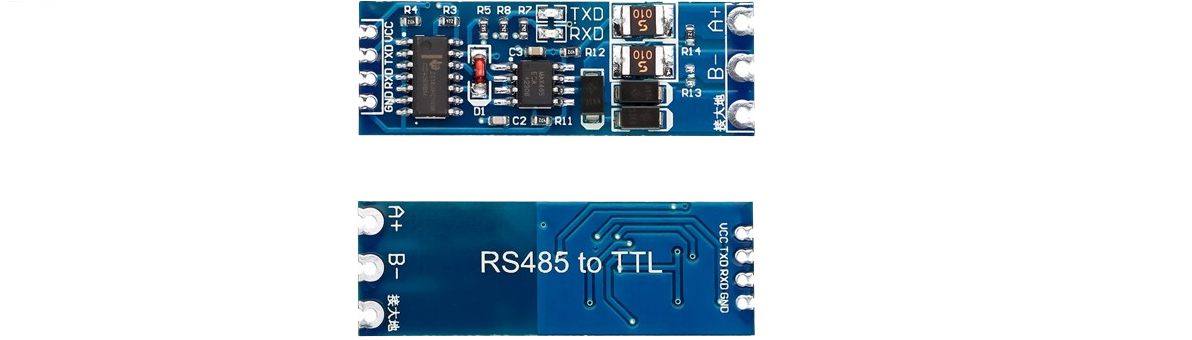
\includegraphics[width=16cm]{figuras/TTL_TO_RS485.png}
    \fonte{Retirado de \textcite{RS485TTL}.}
  \end{varwidth}
\end{figure}

\begin{table}[!htb]
  \caption{Especificações técnicas do Módulo Conversor RS485 para TTL}
  \begin{tabularx}{\textwidth}{|X|X|} \hline
      \textbf{Parâmetro} & \textbf{Detalhes} \\ \hline
      Faixa de operação & 5 V \\ \hline
      Dimensões & 44x14 mm \\ \hline
  \end{tabularx}
  \label{tab:rs485}
  \fonte{Retirado de \textcite{RS485TTL}.}
\end{table}

\subsection{Custos dos Componentes}

Os custos dos componentes utilizados no desenvolvimento desse sistema podem variar de acordo com o fornecedor, região de compra e período de aquisição. A Tabela \ref{tab:custos} apresenta os custos dos componentes utilizados, já com os impostos e taxas de importação inclusos. Os componentes foram comprados por meio da loja virtual \textit{AliExpress} no dia 17/06/2024.

\begin{table}[!htb]
  \caption{Custos dos componentes utilizados no sistema}
  \begin{tabularx}{\textwidth}{|X|X|} \hline
      \textbf{Componente} & \textbf{Custo (R\$)} \\ \hline
      ESP32 & 20,19 \\ \hline
      DHT22 & 7,66 \\ \hline
      BMP280 & 4,65 \\ \hline
      BH1750 & 6,04 \\ \hline
      Anemômetro RS-FSJT-N01 & 100,43 \\ \hline
      LM393 & 4,64 \\ \hline
      NEO-6M & 22,89 \\ \hline
      Conversor RS485 para TTL & 10,86 \\ \hline
      \textbf{Total} & \textbf{177,36} \\ \hline
  \end{tabularx}
  \label{tab:custos}
  \fonte{Elaborado pelo autor, 2024.}
\end{table}


\section{Integração dos sensores ao ESP32}

Como foram utilizados sensores para capturar os dados, é importante destacar que todo instrumento de medição possui erros inerentes \parencite{Vuolo_erro1996}, que podem ser classificados em dois tipos:

\begin{itemize} 
    \item Erros sistemáticos, sendo estes previsíveis e reproduzíveis. Normalmente, são originados de falhas no próprio instrumento de medição ou de influências ambientais que afetam de maneira constante o resultado. Eles podem ser corrigidos através de calibração e ajustes do sistema;
    \item Erros estatísticos, que, diferentemente dos erros sistemáticos, ocorrem de forma aleatória e imprevisível. São, geralmente, causados por flutuações nas condições de medição, como ruído no sinal ou variações no ambiente. Eles não podem ser eliminados por calibração, mas podem ser reduzidos por meio da repetição e tratamento estatístico dos dados. 
\end{itemize}

Neste trabalho, cada sensor passou um teste individual de leitura por um período de 24 horas. Tanto antes quanto depois dos testes, os sensores mantiveram sua operação normal e dentro do esperado de suas especificações técnicas. Isso foi feito a fim de observar e minimizar possíveis erros sistemáticos e garantir o funcionamento ininterrupto dos sensores.

Por fim, os componentes foram integrados em um sistema cyberfísico que publica as leituras individuais de cada sensor em um \textit{broker}. Neste trabalho, optou-se pelo EMQX (Figura \ref{figura:emqx}), uma plataforma de código aberto para MQTT \parencite{EMQX}.

\begin{figure}[!htb] \centering
  \caption{Interface da plataforma EMQX} \label{figura:emqx}
  \begin{varwidth}{\linewidth}
    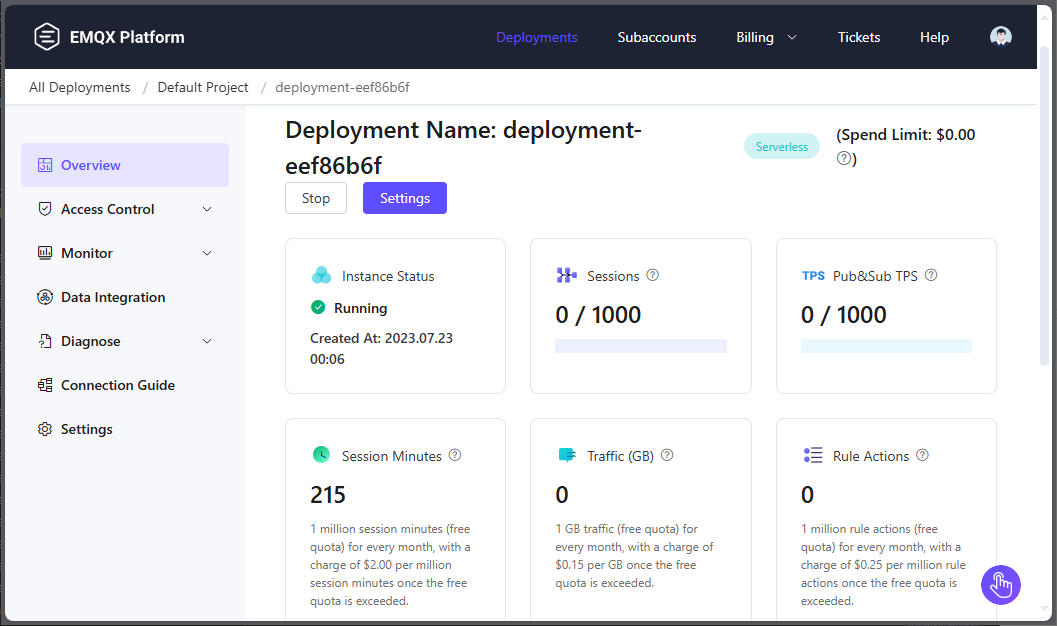
\includegraphics[width=16cm]{figuras/emqx.png}
    \fonte{Elaborado pelo autor, 2024.}
  \end{varwidth}
\end{figure}

Nele, as mensagens são distribuídas em tópicos usando-se protocolos de comunicação (MQTT) e criptografia (TLS). Isso garante a integridade e a confidencialidade dos dados coletados, além do acesso remoto e em tempo real às leituras. Este acesso é feito através da conexão entre o \textit{broker} e o \textit{backend} do sistema, que se inscreve nos tópicos de interesse para receber os dados. Também é feita uma segunda instância de armazenamento em um banco de dados relacional (\textit{MySQL}) para consultas de interesse. 

O armazenamento dos dados históricos no \textit{MySQL} é realizado por meio da funcionalidade de \textit{Rule Engine} do EMQX, que permite criar regras para processar as mensagens recebidas. Por meio dessas regras, as mensagens publicadas nos tópicos são capturadas e inseridas em uma tabela no banco (\texttt{mqtt\_messages}), previamente configurada com colunas \textit{topic}, \textit{payload}, \textit{qos} e \textit{timestamp}. Esse mecanismo permite a persistência dos dados e possibilita consultas históricas para análises ou monitoramento posterior.

\section{Ferramentas e Tecnologias Utilizadas}

Para o desenvolvimento do sistema proposto neste trabalho, foram empregadas ferramentas e tecnologias, cada uma com seus papéis específicos.

\subsection{Linguagem \textit{C}}
A linguagem de programação \textit{C} foi utilizada para o desenvolvimento do \textit{firmware} do ESP32. Essa escolha deve-se à sua proximidade com o \textit{hardware}, permitindo maior controle sobre os recursos embarcados. Além disso, o \textit{C} é suportado nativamente por diversas plataformas de desenvolvimento, o que facilita a portabilidade do código.

No desenvolvimento do \textit{firmware}, diversas bibliotecas foram empregadas para simplificar a implementação e assegurar a confiabilidade das funcionalidades. Abaixo, são listadas as principais bibliotecas utilizadas:

\begin{itemize}
    \item \texttt{Arduino}: biblioteca base para desenvolvimento com a plataforma Arduino, fornecendo funções para manipulação de pinos, comunicação serial e temporização.
    \item \texttt{ModbusMaster}: implementação do protocolo Modbus RTU, permitindo comunicação entre dispositivos escravos e mestres em redes industriais.
    \item \texttt{Wire}: biblioteca utilizada para comunicação I2C, facilitando a integração com sensores e dispositivos externos.
    \item \texttt{WiFi}: biblioteca nativa para gerenciar conexões Wi-Fi no ESP32, necessária para conectividade com redes locais e a \textit{internet}.
    \item \texttt{Adafruit\_Sensor} e \texttt{Adafruit\_BMP280}: fornecem suporte para leitura de dados ambientais de sensores como o BMP280, usado para medir pressão atmosférica e temperatura.
    \item \texttt{DHT} e \texttt{DHT\_U}: bibliotecas dedicadas a sensores de temperatura e umidade da linha DHT (por exemplo, DHT11 ou DHT22).
    \item \texttt{BH1750}: biblioteca para integração com o sensor de luz BH1750, utilizado para medições de luminosidade.
    \item \texttt{WiFiClientSecure}: extensão da biblioteca Wi-Fi para conexões utilizando TLS/SSL, garantindo comunicações criptografadas.
    \item \texttt{PubSubClient}: implementação do protocolo MQTT, necessário para a comunicação com o \textit{backend}.
    \item \texttt{TinyGPSPlus}: biblioteca para interpretação de dados recebidos de módulos GPS, necessários para obter informações de localização geográfica.
\end{itemize}

A combinação dessas bibliotecas permitiu a criação de um \textit{firmware} capaz de monitorar e controlar diversos sensores e atuadores, além de garantir conectividade e comunicação com sistemas externos.

\subsection{\textit{Node.js}}
O ambiente de execução \textit{Node.js} foi empregado no desenvolvimento do \textit{backend} devido à sua capacidade de gerenciar múltiplas conexões simultâneas. \textit{Node.js} é particularmente adequado para aplicações que exigem baixa latência, como em sistemas em tempo real.

No desenvolvimento do \textit{backend}, foram usadas diversas bibliotecas para otimizar funcionalidades e assegurar boas práticas de programação. A seguir, são destacadas as principais dependências e suas funções no projeto:

\begin{itemize}
    \item \texttt{Express}: \textit{Framework} para construção de servidores \textit{web}, usado para gerenciar rotas e requisições HTTP.
    \item \texttt{Axios}: Biblioteca empregada para realizar requisições HTTP, facilitando a comunicação com APIs externas.
    \item \texttt{Cors}: \textit{Middleware} que permite configurar políticas de compartilhamento de recursos entre diferentes origens, necessário para integrar o \textit{frontend} com o \textit{backend}.
    \item \texttt{Dotenv}: biblioteca usada para gerenciar variáveis de ambiente, permitindo a configuração de credenciais e configurações do sistema.
    \item \texttt{MQTT}: protocolo para comunicação em tempo real, empregado no gerenciamento de mensagens entre dispositivos conectados.
    \item \texttt{Zod}: biblioteca para validação e definição de esquemas de dados, assegurando a integridade das entradas e saídas da aplicação.
\end{itemize}

Além das dependências de produção, foi utilizada uma estrutura de dependências de desenvolvimento para garantir qualidade no código e simplificar o processo:

\begin{itemize}
    \item \texttt{Typescript}: \textit{Superset} do JavaScript que adiciona tipagem estática ao código, prevenindo erros.
    \item \texttt{Jest} e \texttt{Supertest}: ferramentas para testes automatizados que permitem validar funcionalidades e garantir o funcionamento correto da aplicação.
    \item \texttt{ESLint} e \texttt{Prettier}: configurações para impor boas práticas de codificação e formatação consistente, otimizando a legibilidade e manutenção do código.
    \item \texttt{Nodemon} e \texttt{ts-node}: facilitam o desenvolvimento ao permitir recarga automática do servidor e execução de arquivos TypeScript sem necessidade de transpilação prévia.
\end{itemize}

Esse conjunto de ferramentas proporcionou um ambiente de desenvolvimento produtivo e um \textit{backend} eficiente, escalável e seguro.

\subsection{\textit{Next.js}}
A biblioteca \textit{Next.js} foi utilizada para o desenvolvimento da interface do \textit{frontend}, oferecendo uma arquitetura de renderização híbrida que combina renderização do lado do servidor - SSR (sigla do inglês, \textit{server-side rendering}) e renderização do lado do cliente - CSR (sigla do inglês, \textit{client-side rendering}). Isso permite que as páginas \textit{web} sejam renderizadas no servidor e enviadas para o cliente, proporcionando uma experiência de usuário rápida e responsiva. A seguir, destacam-se as principais dependências empregadas no projeto e suas funcionalidades:

\begin{itemize} 
  \item \texttt{@next/font}: utilizado para integrar fontes personalizadas diretamente no projeto, otimizando o desempenho no carregamento de fontes. 
  \item \texttt{@radix-ui/react-dropdown-menu}, \texttt{@radix-ui/react-scroll-area} e \texttt{@radix-ui/react-slot}: componentes acessíveis e estilizados para construção de interfaces reativas e intuitivas.
  \item \texttt{@tailwindcss/typography}: \textit{Plugin} do \textit{TailwindCSS} que adiciona estilos predefinidos para tipografia, simplificando a criação de layouts bem formatados. 
  \item \texttt{axios}: biblioteca utilizada para realizar requisições HTTP, integrando a interface com as APIs do \textit{backend}. 
  \item \texttt{class-variance-authority}: facilita a manipulação de classes CSS com base em variantes condicionais, permitindo maior flexibilidade no estilo. 
  \item \texttt{clsx}: utilizado para combinar classes CSS dinamicamente, de maneira concisa e legível. 
  \item \texttt{lucide-react}: biblioteca de ícones leves e modernos, utilizada para enriquecer a interface visual. 
  \item \texttt{next-themes}: fornece suporte à alternância entre temas claros e escuros, aprimorando a experiência do usuário. 
  \item \texttt{react-icons}: conjunto abrangente de ícones para \textit{React}, permitindo a inclusão de gráficos contextuais no \textit{design}. 
  \item \texttt{react-responsive-carousel}: componente de carrossel responsivo para exibição de imagens ou conteúdos de forma dinâmica. 
  \item \texttt{sharp}: biblioteca para manipulação de imagens no lado do servidor, otimizando tamanhos e formatos para diferentes dispositivos. 
  \item \texttt{tailwind-merge}: facilita a mesclagem de classes \textit{TailwindCSS}, ajudando a resolver conflitos de estilo. 
  \item \texttt{tailwindcss-animate}: \textit{Plugin} que adiciona animações ao \textit{TailwindCSS}, tornando a experiência do usuário mais fluida e atraente. 
  \item \texttt{zod}: biblioteca para validação e definição de esquemas de dados, assegurando a integridade das informações manipuladas no \textit{frontend}. \end{itemize}

Para garantir qualidade e consistência durante o desenvolvimento, foram empregadas diversas dependências de ambiente:

\begin{itemize} 
  \item \texttt{@types/node}, \texttt{@types/react} e \texttt{@types/react-dom}: adicionam tipagem para as bibliotecas principais, garantindo integração com o \texttt{Typescript}. 
  \item \texttt{autoprefixer}: automatiza a inclusão de prefixos de compatibilidade para navegadores, assegurando suporte abrangente ao CSS. 
  \item \texttt{eslint} e \texttt{eslint-config-next}: ferramentas de análise de código estático que impõem boas práticas no desenvolvimento. 
  \item \texttt{eslint-config-prettier}: garante integração entre o \texttt{ESLint} e o \texttt{Prettier}, evitando conflitos entre as regras. 
  \item \texttt{postcss}: Processador CSS que melhora a compatibilidade e otimização dos estilos. 
  \item \texttt{prettier}: ferramenta de formatação automática, assegurando consistência visual no código. 
  \item \texttt{tailwindcss}: \textit{Framework} de utilitários CSS que acelera o desenvolvimento de estilos responsivos e customizados. 
  \item \texttt{typescript}: adiciona tipagem estática ao JavaScript, prevenindo erros comuns e proporcionando maior robustez ao código. \end{itemize}

Esse conjunto de ferramentas e dependências permitiu o desenvolvimento de um \textit{frontend} moderno, dinâmico e escalável, com foco na experiência do usuário e na eficiência do sistema.

\subsection{\textit{Jest}}
O \textit{framework} de testes \textit{Jest} foi adotado para a realização de testes automatizados. Essa ferramenta foi escolhida por sua simplicidade de configuração e pela capacidade de executar testes unitários e de integração, garantindo a qualidade e a confiabilidade do código, além de facilitar a manutenção e evolução do sistema.

A estrutura dos testes foi organizada em dois principais níveis, separados por pastas, para maior clareza e modularidade:

\begin{itemize}
  \item Ponta a ponta: contém testes que verificam o funcionamento completo da aplicação em cenários reais, cobrindo desde as requisições feitas ao servidor até as respostas entregues. No sistema implementado nesta pesquisa, o teste avalia o comportamento do sistema como um todo, validando o fluxo de dados entre os componentes.
  \item Unitários: reúne testes focados em unidades específicas do sistema, como funções, serviços ou classes individuais. Cada teste nesta pasta avalia o comportamento isolado de componentes-chave, garantindo que funcionem conforme o esperado. Nesta pesquisa, os testes unitários foram utilizados para validar a lógica de negócio e o transporte dos dados entre as camadas do sistema.
\end{itemize}

Essa organização entre testes de integração e testes unitários permite isolar falhas e assegurar que tanto os componentes individuais quanto a aplicação como um todo funcionem de forma consistente e modular.

\subsection{\textit{Shadcn/ui}}
A biblioteca de componentes \textit{Shadcn/ui} foi utilizada no desenvolvimento do \textit{frontend}, proporcionando componentes reutilizáveis e estilizados que aceleraram o processo de construção da interface. Essa biblioteca foi selecionada por sua flexibilidade e integração nativa com o \textit{framework} \textit{TailwindCSS}. Neste trabalho, foram usados os seguintes componentes:
\begin{itemize}
  \item \texttt{Button}: botão interativo com estilos personalizáveis e animações integradas.
  \item \texttt{Badge}: indicador visual para destacar informações importantes.
  \item \texttt{Card}: cartão de conteúdo com layout flexível e responsivo.
  \item \texttt{Dropdown-menu}: menu suspenso com opções personalizáveis e animações suaves.
  \item \texttt{Scroll-area}: área de rolagem personalizada com suporte a conteúdo dinâmico.
  \item \texttt{Skeleton}: efeito de carregamento para indicar que o conteúdo está sendo carregado.
\end{itemize}

\subsection{\textit{TailwindCSS}}
O \textit{framework} \textit{TailwindCSS} foi empregado na estilização do \textit{frontend}. Sua abordagem utilitária permite a criação de interfaces consistentes e bem estilizadas de maneira rápida e eficiente, o que foi importante para garantir um \textit{design} responsivo e atrativo. Neste travalho, foram utilizadas paletas de cores voltadas para o uso em ambientes externos, com tons de verde e branco destacados.

\subsection{Figma}
A ferramenta Figma (Figura \ref{figura:figma}) foi empregada na prototipagem de interfaces gráficas. Sua escolha foi motivada pela variedade de recursos disponíveis para o \textit{design} e validação de interfaces antes de sua implementação.

\begin{figure}[!htb] \centering
  \caption{Interface da aplicação Figma} \label{figura:figma}
  \begin{varwidth}{\linewidth}
    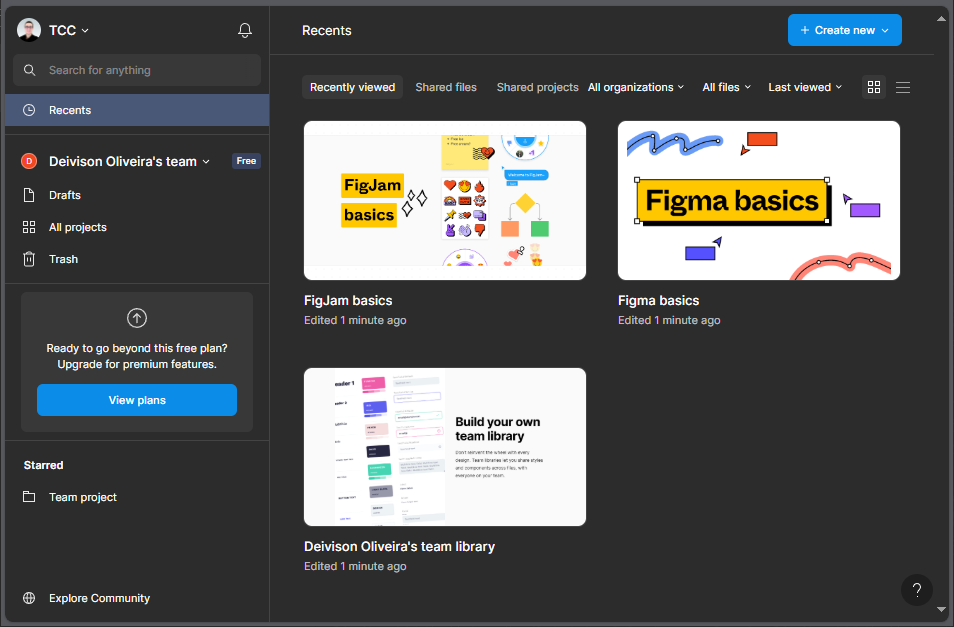
\includegraphics[width=16cm]{figuras/figma.png}
    \fonte{Elaborado pelo autor, 2024.}
  \end{varwidth}
\end{figure}

\subsection{Visual Studio Code}
O Visual Studio Code (Figura \ref{figura:vscode}) foi empregado como ambiente de desenvolvimento integrado - IDE (sigla do inglês \textit{Integrated Development Environment}) para o desenvolvimento do \textit{frontend} e do \textit{backend}. Essa ferramenta foi escolhida por sua versatilidade, extensibilidade e suporte a diversas linguagens e tecnologias, incluindo as mencionadas neste trabalho.

\begin{figure}[!htb] \centering
  \caption{Interface do Visual Studio Code} \label{figura:vscode}
  \begin{varwidth}{\linewidth}
    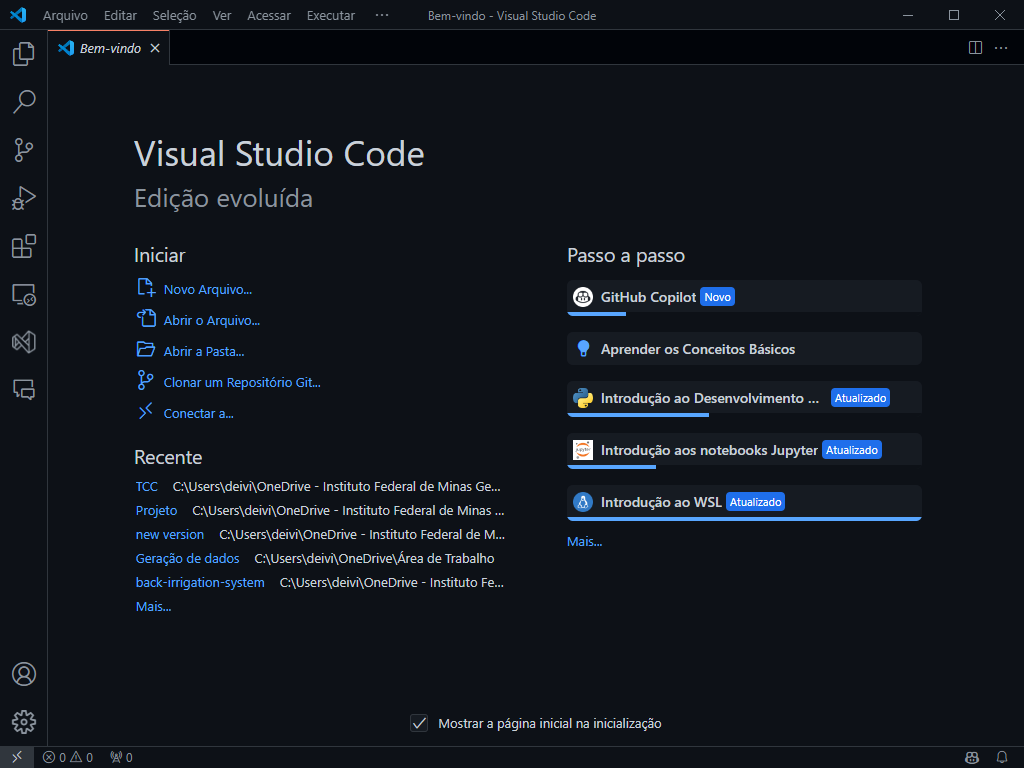
\includegraphics[height=10cm, width=16cm]{figuras/vscode.png}
    \fonte{Elaborado pelo autor, 2024.}
  \end{varwidth}
\end{figure}

\subsection{Arduino IDE}
A Arduino IDE (Figura \ref{figura:arduino-ide}) foi utilizada como IDE para o desenvolvimento embarcado no ESP32. Essa escolha se justifica pela usabilidade da ferramenta e pela compatibilidade com a plataforma ESP32, facilitando a criação e a depuração do \textit{firmware}.

\begin{figure}[!htb] \centering
  \caption{Interface do Arduino IDE} \label{figura:arduino-ide}
  \begin{varwidth}{\linewidth}
    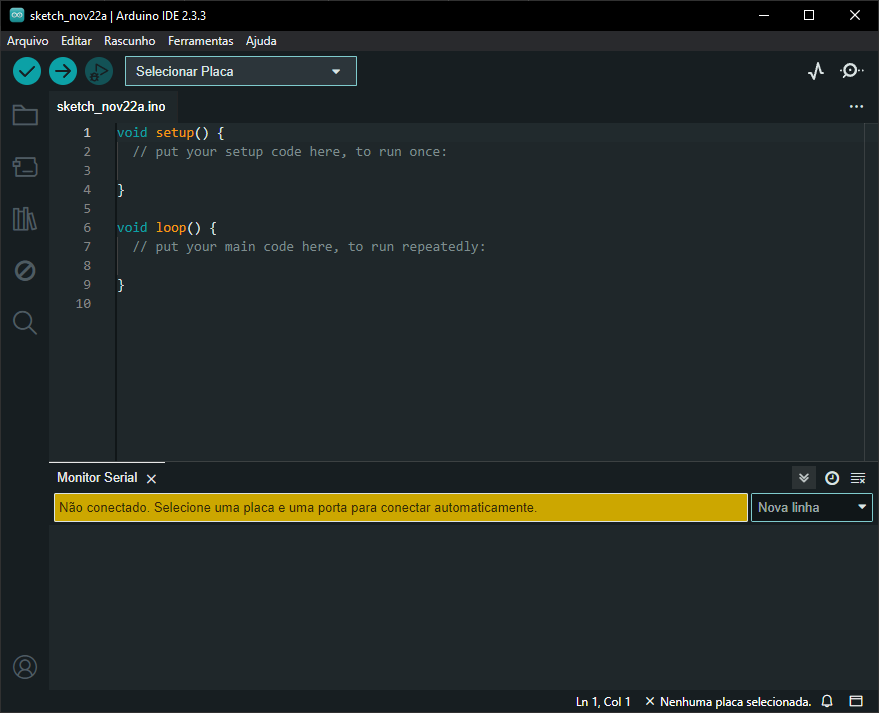
\includegraphics[height=10cm, width=16cm]{figuras/arduino-ide.png}
    \fonte{Elaborado pelo autor, 2024.}
  \end{varwidth}
\end{figure}

\subsection{Fritzing}
O Fritzing (Figura \ref{figura:fritzing}) foi empregado na prototipagem de circuitos eletrônicos. Essa ferramenta permite a criação de esquemas e \textit{layouts} de circuitos de maneira intuitiva, sendo necessária para a validação do \textit{hardware} antes de sua implementação definitiva.

\begin{figure}[!htb] \centering
  \caption{Interface da aplicação Fritzing} \label{figura:fritzing}
  \begin{varwidth}{\linewidth}
    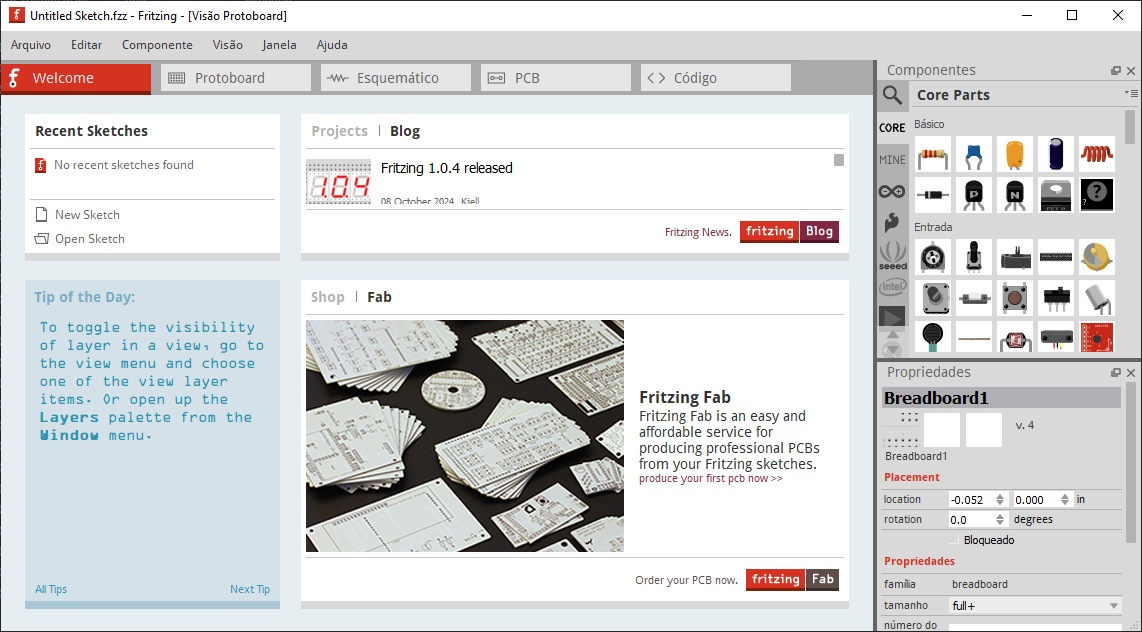
\includegraphics[width=16cm]{figuras/fritzing.png}
    \fonte{Elaborado pelo autor, 2024.}
  \end{varwidth}
\end{figure}

\subsection{EasyEDA}
A ferramenta EasyEDA (Figura \ref{figura:easyeda}) foi utilizada para o desenho das placas de circuito impresso - PCB (sigla do inglês \textit{Printed Circuit Board}). Sua escolha foi motivada pela facilidade de uso e pelos recursos para simulação e validação de projetos eletrônicos, garantindo a qualidade e a confiabilidade das placas desenvolvidas.

\begin{figure}[!htb] \centering
  \caption{Interface da aplicação EasyEDA} \label{figura:easyeda}
  \begin{varwidth}{\linewidth}
    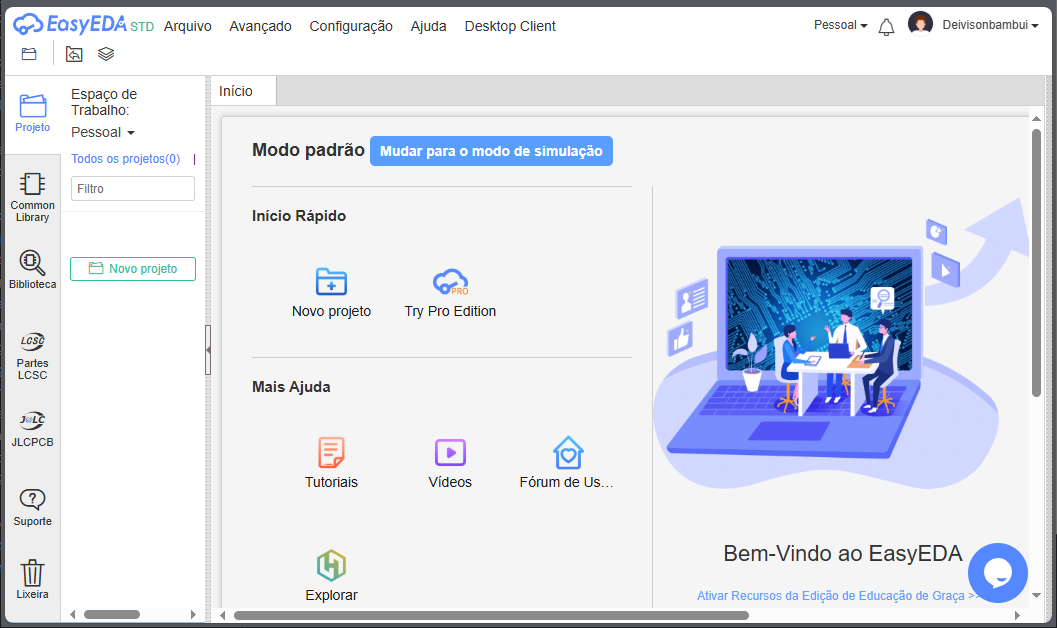
\includegraphics[width=16cm]{figuras/easyeda.png}
    \fonte{Elaborado pelo autor, 2024.}
  \end{varwidth}
\end{figure}

\subsection{Resumo das escolhas}
As tecnologias e ferramentas mencionadas foram selecionadas para atender aos requisitos específicos do sistema proposto, priorizando desempenho, escalabilidade e experiência prévia de desenvolvimento.

A análise dos dados meteorológicos é realizada de forma contínua para apresentar medições e cálculos estimativos de ETo e ETc locais. Esse método de análise permite a interpretação e avaliação dos dados de forma rápida, além de gerar relatórios periódicos para a tomada de decisões.

\section{Estimativa da evapotranspiração}

O cálculo da ETo e da ETc é usado para o monitoramento hídrico em tempo real e é realizado com base nas leituras dos sensores. Foram usadas as equações da FAO-56 apresentadas por \textcite{Allen_evapotranspiration1998} como modelagem referencial. Cada leitura dos sensores contribui diretamente para o cálculo dessas variáveis, ou é convertida de forma a ser utilizada na equação.

\subsection{Variáveis meteorológicas e sua obtenção}

As variáveis meteorológicas utilizadas no cálculo da evapotranspiração são obtidas da seguinte forma:
\begin{itemize}
    \item A temperatura do ar (\(T\)) é medida diretamente do sensor DHT22, que fornece a temperatura em graus Celsius;
    
    \item A umidade relativa (\(RH\)) também é medida pelo sensor DHT22, em percentual;
    
    \item A umidade do solo (\(h\)) é medida pelo comparador LM393 com eletrodos externos, em um intervalo analógico;
    
    \item A pressão atmosférica (\(P\)) é obtida do sensor BMP280, em hPa;

    \item A velocidade do vento (\(u_2\)) é medida pelo anemômetro, em m/s.
\end{itemize}

As demais variáveis são estimadas a partir de cálculos intermediários, obtidos, em sua maioria, da obra de \textcite{Allen_evapotranspiration1998}:
\begin{itemize}
    \item A radiação líquida (\(R_n\)) é estimada a partir das leituras do sensor de luminosidade BH1750, que mede a intensidade luminosa em lux a cada segundo. 
    \begin{itemize}
        \item \textcite{Michael_2020} apresentam a conversão de lux (\(lx\)) para irradiância solar (\(E\)) em W/m², dada pela equação:
        \[ E \approx \frac{lx}{120} \]

        \item A irradiância solar, por sua vez, é a própria radiação solar (\(R_s\)):
        
        \[ R_s = E \]

        \item Desta forma, é possível determinar a radiação líquida solar (\(R_{ns}\)), dada por:
        
        \[ R_{ns} = 0.77 \cdot R_s \]

        \item O último componente necessário para determinar a \(R_n\) é a radiação líquida de ondas longas (\(R_{nl}\)), que é resultante das seguintes equações:
        
        \begin{itemize}
            \item A distância relativa inversa Terra-Sol (\(d_r\)), que é calculada como:
            
            \[
            d_r = 1 + 0.033 \cos\left( \frac{2 \pi J}{365} \right)
            \]
            onde \(J\) é o dia do ano.
            
            \item A radiação extraterrestre por períodos horários ou mais curtos (\(R_a\)), dada por:
            
            \[
            R_a = \frac{12 \cdot 60}{\pi} G_{sc} d_r 
            \left[ 
            (\omega_2 - \omega_1) \sin(\phi) \sin(\delta) + 
            \cos(\phi) \cos(\delta) (\sin(\omega_2) - \sin(\omega_1)) 
            \right]
            \]
            onde \(G_{sc} = 0.0820 \, MJ \, m^{-2} \, min^{-1}\), \( \delta = 0.409 \sin\left( \frac{2 \pi J}{365} - 1.39 \right)\), \(\phi\) é o grau de latitute (obtido pelo módulo GPS NEO-6M V2), e os ângulos \( \omega_1 \) e \( \omega_2 \) são os ângulos de tempo solar no início e no final do período, respectivamente.
            
            \item A radiação solar com céu limpo (\(R_{so}\)), dada por:
            
            \[
            R_{so} = (0.75 + 2 \cdot 10^{-5} z) R_a
            \]
            onde \(z\) é a elevação, em metros, do nível do mar.
            
            \item A radiação líquida de ondas longas (\(R_{nl}\)), estimada por:
            
            \[
            R_{nl} = \sigma \left( \frac{T_{max,K}^4 + T_{min,K}^4}{2} \right) \left[ 0.34 - 0.14 \sqrt{e_a} \right] \left( 1.35 \frac{R_s}{R_{so}} - 0.35 \right)
            \]
            onde \(T_{max,K}\) e \(T_{min,K}\) são as temperaturas máxima e mínima em Kelvin, \( \sigma \) é a constante de Stefan-Boltzmann (\(4.903 \cdot 10^{-9} \, MJ \, K^{-4} \, m^{-2} \, dia^{-1} \)), e \(e_a\) é a pressão de vapor atual.
        \end{itemize}

        \item A \(R_n\) resultante é dada por:
        
        \[ R_n = R_{ns} - R_{nl} \]
    \end{itemize}
    
    \item A variação da pressão de saturação (\(\Delta\)) é calculada com a equação:
    \[
    \Delta = \frac{4098 \cdot (0.6108 \cdot e^{\frac{17.27 \cdot T}{T + 237.3}})}{(T + 237.3)^2}
    \]
    
    \item A pressão de saturação (\(e_s\)) é calculada usando-se:
    \[
    e_s = \frac{0.6108 \cdot e^{\frac{17.27 \cdot T_{max}}{T_{max} + 237.3}} + 0.6108 \cdot e^{\frac{17.27 \cdot T_{min}}{T_{min} + 237.3}}}{2}
    \]
    
    \item A pressão de vapor atual (\(e_a\)) é obtida com:
    \[
    e_a = 0.6108 \cdot e^{\frac{17.27 \cdot T}{T + 237.3}}
    \]
    
    \item O fluxo de calor do solo (\(G\)) é definido pela hora, ou seja, considera-se: \(G = 0.1 \cdot R_n\) durante o dia e \(G = 0.5 \cdot R_n\) durante a noite;
    
    \item A constante psicrométrica (\(\gamma\)) é dada por:
    \[
    \gamma = 0.665 \cdot 10^{-3} \cdot P
    \]
    onde \(P\) é a pressão atmosférica, fornecida pelo sensor BMP280.
\end{itemize}

No sistema proposto, cada variável listada acima, seja ela medida diretamente ou calculada, é apresentada no painel da aplicação \textit{web}. Variáveis obtidas diretamente são aquelas cujos sensores têm sua leitura publicada em tópicos MQTT. Já as calculadas são obtidas a partir de manipulações dessas leituras. Isso é feito por um dos \textit{use-cases} do \textit{backend}, que é responsável por calcular e disponibilizar as variáveis em \textit{endpoints} que são consumidos pelo \textit{frontend}. Também há um tópico de MQTT para publicação de erros e alertas que são gerados a partir de condições específicas. Os erros cobertos incluem valores fora de faixa de leitura esperada, falhas de comunicação (tanto Wi-fi quanto no \textit{broker} MQTT) ou falhas de \textit{hardware} do ESP32.

\section{Desenvolvimento da aplicação}
Nesta subseção, são apresentados os detalhes do desenvolvimento da aplicação, incluindo a arquitetura do sistema e os métodos de prototipagem utilizados.

\subsection{Padrões arquiteturais e práticas utilizadas}

No desenvolvimento do sistema, foram adotados padrões arquiteturais para garantir a modularidade, escalabilidade e manutenção do código. A arquitetura foi baseada nos princípios de \textit{Domain-Driven Design} (DDD) e nos cinco princípios SOLID \parencite{ddd_eric2004}.

O DDD foi escolhido como base para a estruturação do sistema devido à sua capacidade de refletir a complexidade do domínio meteorológico no código. A aplicação foi dividida em camadas como \textit{domain}, \textit{application}, \textit{infrastructure} e \textit{interfaces}, em que cada uma possui responsabilidades bem definidas. Isso facilita a evolução e a adaptação do sistema a novos requisitos.

Os princípios SOLID foram aplicados para garantir um código coeso, desacoplado e extensível. Especificamente:
\begin{itemize}
    \item O princípio da responsabilidade única (SRP) foi adotado para garantir que cada classe ou módulo tenha uma única responsabilidade, facilitando a manutenção e evolução do código;
    \item O princípio aberto/fechado (OCP) assegurou que os componentes do sistema fossem abertos para extensão, mas fechados para modificação, permitindo a adição de novas funcionalidades sem alterar o código existente;
    \item O princípio da substituição de Liskov (LSP) foi utilizado para garantir que as classes derivadas pudessem substituir suas classes-base sem alterar o comportamento do sistema;
    \item O princípio da segregação de interfaces (ISP) assegurou que as interfaces fossem específicas para cada tipo de cliente, evitando a implementação de métodos desnecessários;
    \item O princípio da inversão de dependência (DIP) foi seguido para garantir que módulos de alto nível não dependessem de módulos de baixo nível, mas sim de abstrações, promovendo o desacoplamento do código.
\end{itemize}

Essas práticas resultaram em um código mais limpo, testável e resiliente, capaz de suportar a evolução contínua do sistema sem comprometer sua integridade.

\subsection{Ciclo de desenvolvimento do software}

O ciclo de desenvolvimento do \textit{software} envolveu tanto a parte \textit{web} quanto a embarcada, seguindo uma abordagem iterativa e incremental. Foi utilizado o \textit{Git Workflow} como estratégia principal de controle de versões \parencite{pro_git}.

Para o desenvolvimento \textit{web}, o fluxo começou com a definição dos requisitos e a modelagem do domínio, seguida pela implementação das funcionalidades em \textit{branches} específicas, alinhadas com as funcionalidades do sistema. Cada \textit{feature branch} era integrada à \textit{branch develop} após a aprovação em revisões de código e a passagem pelos testes automatizados, garantindo a qualidade e a integração contínua do código. O \textit{Git Workflow} utilizado incluiu a criação de \textit{feature branches}, \textit{hotfix branches} e \textit{release branches}, de acordo com o estado de desenvolvimento e manutenção do sistema.

Para o desenvolvimento embarcado, foram utilizados ciclos mais curtos, devido à necessidade de validação rápida dos sensores e componentes físicos. Cada ciclo incluiu a configuração do \textit{hardware}, a programação do \textit{firmware} no ESP32 utilizando a Arduino IDE e testes físicos para validação dos dados coletados. As versões do código embarcado eram gerenciadas em um repositório \textit{Git} separado, seguindo uma estrutura similar à usada para o desenvolvimento \textit{web}. Nesse caso, foram feitas adaptações para as necessidades específicas do desenvolvimento embarcado, incluindo a verificação de integrações entre sensores e o envio dos dados ao \textit{broker} EMQX.

A sinergia entre essas duas frentes de desenvolvimento foi usada para garantir que o sistema operasse de forma coesa e integrada, desde a captura dos dados até a sua visualização na interface \textit{web}.

\subsection{Prototipagem e distribuição dos componentes}

A prototipagem do sistema foi uma etapa importante para garantir que os componentes de \textit{hardware} e \textit{software} funcionassem harmoniosamente. O processo começou com a criação de protótipos funcionais simples, utilizando-se o \textit{Fritzing} para o \textit{design} dos circuitos e a prototipagem das interações entre os sensores e o microcontrolador ESP32.

O desenvolvimento do protótipo envolveu a montagem dos sensores em uma \textit{breadboard}, permitindo ajustes rápidos e trocas de componentes conforme necessário. O \textit{layout} dos componentes foi projetado no EasyEDA de forma a otimizar a coleta de dados, minimizando interferências e garantindo a precisão das medições (Figura \ref{figura:pcb-layout}). 

Após a validação do protótipo inicial, os componentes foram instalados em uma montagem permanente. Isso foi feito utilizando-se uma PCB e cabos para alimentação e comunicação com sensores externos. A PCB foi usinada com base no \textit{layout} exportado do EasyEDA (Figura \ref{figura:pcb-scheme}), sendo feita uma matriz para as trilhas e furos necessários (Figura \ref{figura:pcb-matriz}). A usinagem foi feita usando-se percloreto de ferro sobre uma placa de fenolite, tendo a matriz impressa sobre a placa e a corrosão feita com o percloreto (Figura \ref{figura:pcb-pos}). Após a corrosão, limpou-se a placa, e os furos foram feitos com uma broca de 1 mm (Figura \ref{figura:pcb-stg1}).

\newpage

\begin{figure}[!htb] \centering
  \caption{\textit{Layout} do protótipo} \label{figura:pcb-layout}
  \begin{varwidth}{\linewidth}
    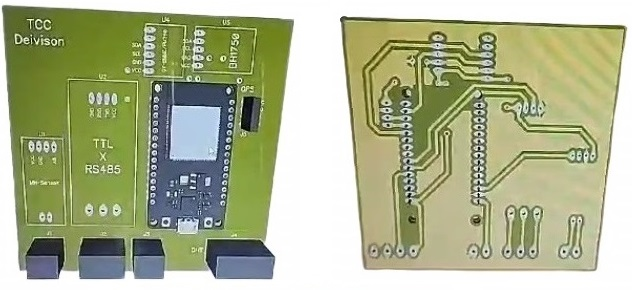
\includegraphics[width=16cm]{figuras/prototype-pcb.jpg}
    \fonte{Elaborado pelo autor, 2024.}
  \end{varwidth}
\end{figure}

\begin{figure}[!htb] \centering
  \caption{Matriz exportada do EasyEDA} \label{figura:pcb-scheme}
  \begin{varwidth}{\linewidth}
    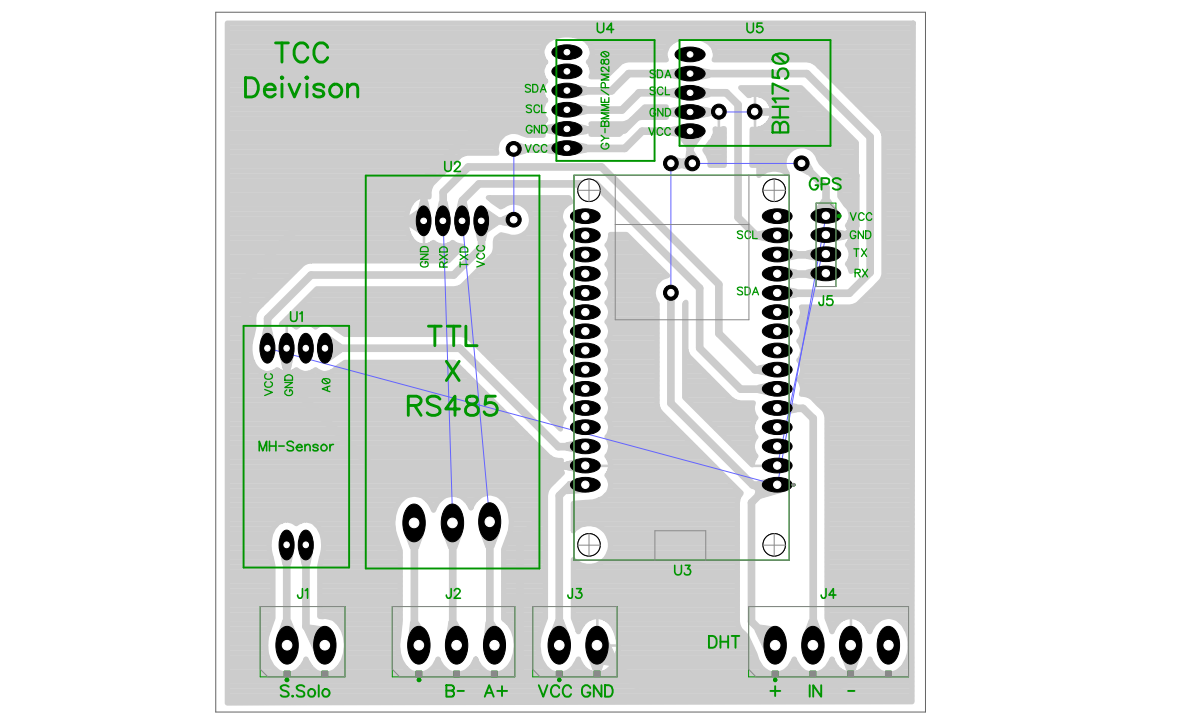
\includegraphics[width=16cm]{figuras/pcb-scheme.png}
    \fonte{Elaborado pelo autor, 2024.}
  \end{varwidth}
\end{figure}

\begin{figure}[!htb] \centering
  \caption{Matriz impressa em papel-filme} \label{figura:pcb-matriz}
  \begin{varwidth}{\linewidth}
    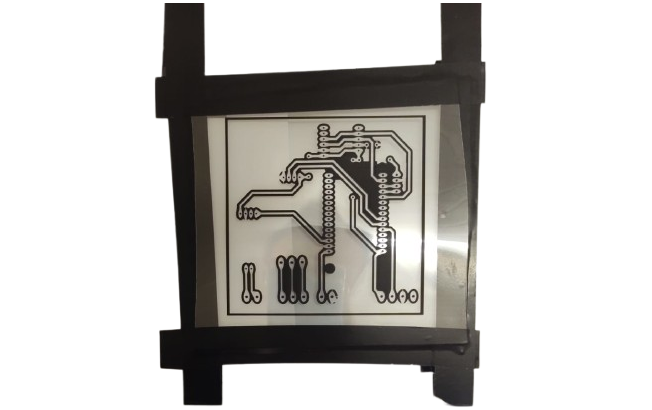
\includegraphics[width=16cm]{figuras/pcb-matriz.png}
    \fonte{Elaborado pelo autor, 2024.}
  \end{varwidth}
\end{figure}

\newpage

\begin{figure}[!htb] \centering
  \caption{PCB finalizada} \label{figura:pcb-pos}
  \begin{varwidth}{\linewidth}
    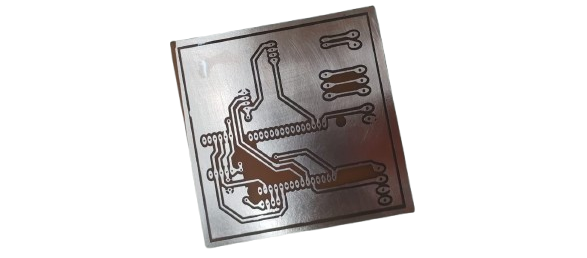
\includegraphics[width=16cm]{figuras/pcb-pos.png}
    \fonte{Elaborado pelo autor, 2024.}
  \end{varwidth}
\end{figure}

\begin{figure}[!htb] \centering
  \caption{PCB pós-corrosão} \label{figura:pcb-stg1}
  \begin{varwidth}{\linewidth}
    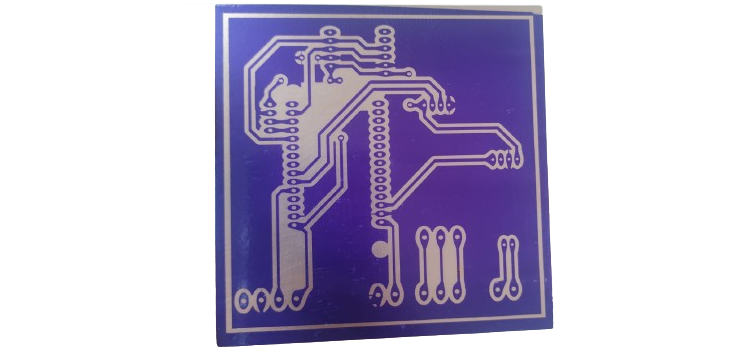
\includegraphics[width=16cm]{figuras/pcb-stg1.png}
    \fonte{Elaborado pelo autor, 2024.}
  \end{varwidth}
\end{figure}

\newpage

Para a prototipagem do \textit{software}, foram utilizados \textit{mockups} e \textit{wireframes} para definir as interfaces e fluxos de usuário. Ferramentas como \textit{Figma} foram empregadas para criar protótipos das telas, que serviram de guia para o desenvolvimento do \textit{frontend} em \textit{Next.js}. A distribuição dos componentes de \textit{software} seguiu o princípio de modularidade, permitindo que cada módulo fosse desenvolvido e testado isoladamente antes de ser integrado ao sistema principal.

A metodologia adotada permitiu uma transição suave do protótipo para a implementação final, garantindo que todos os componentes do sistema fossem adequadamente validados e integrados antes da implantação no laboratório.